\section{Growth of Satellite Constellations} \label{sec:satellite-constellations}

Recent years saw a rapid development of satellite technology, especially due to the growing demand of global connectivity and communication.
Therefore, companies constructed their own satellite constellations leading to a total number of more than 29'000 objects in space at the time of writing.

\begin{figure}[ht]
	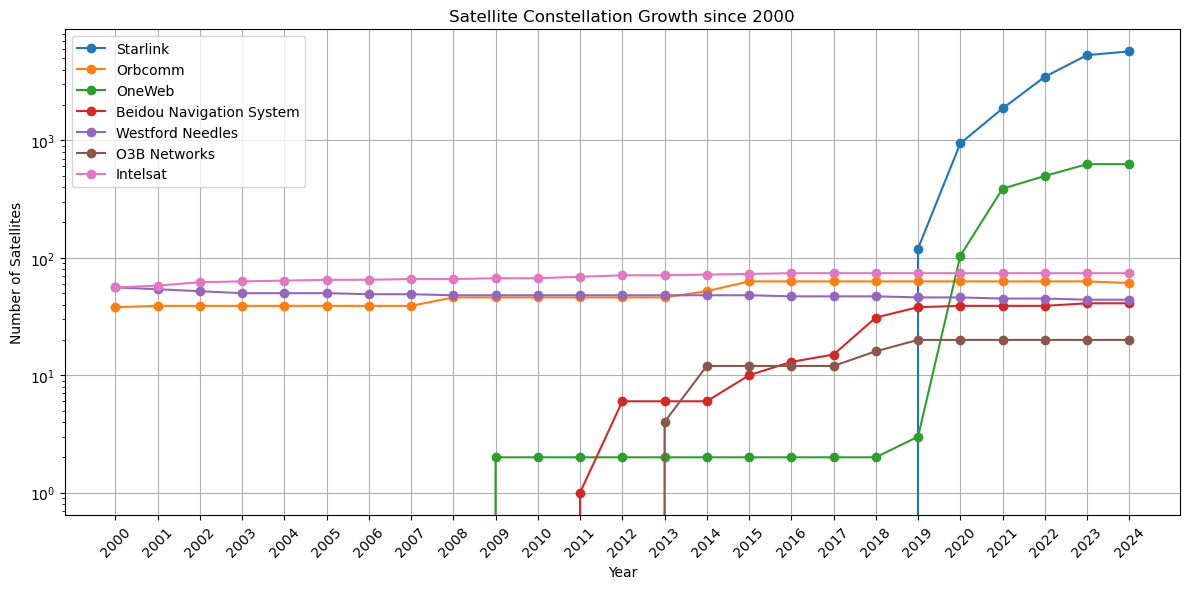
\includegraphics[width=\textwidth]{./chapters/4-results/satellites/img/sattelite-dev.png}
	\caption{Growth of number of satellites in different satellite constellation from 2000 to 2024.\footnote{Note the logarithmic scale.}}
	\label{fig:growth-satellite-constellations}
\end{figure}

\begin{table}
	\caption{Growth of satellite constellations from 2017 to 2024}
	\label{fig:satellite-constellations-short}
	\begin{tabular}{lrrrrrrrr}
		\toprule
		                          & 2017 & 2018 & 2019 & 2020 & 2021 & 2022 & 2023 & 2024 \\
		Classification            &      &      &      &      &      &      &      &      \\
		\midrule
		\textbf{Starlink}         & 0    & 0    & 120  & 943  & 1871 & 3481 & 5326 & 6396 \\
		\textbf{Orbcomm}          & 63   & 63   & 63   & 63   & 63   & 63   & 63   & 61   \\
		\textbf{OneWeb}           & 2    & 2    & 3    & 104  & 388  & 498  & 628  & 628  \\
		\textbf{Beidou}           & 15   & 31   & 38   & 39   & 39   & 39   & 41   & 41   \\
		\textbf{Westford Needles} & 47   & 47   & 46   & 46   & 45   & 45   & 44   & 44   \\
		\textbf{O3B Networks}     & 12   & 16   & 20   & 20   & 20   & 20   & 20   & 20   \\
		\textbf{Intelsat}         & 74   & 74   & 74   & 74   & 74   & 74   & 74   & 74   \\
		\bottomrule
	\end{tabular}
\end{table}


Figure~\ref{fig:growth-satellite-constellations} shows various satellite constellations with the number of satellites per year. Table~\ref{fig:satellite-constellations-short} show the corresponding numbers, starting in 2015 \cite{Richter2024}.
One can see that Starlink is by far the constellation with most satellites.
At the time of writing, it has 6'396 satellites. Starlink grew from 2022 to 2023 by nearly 2000 satellites.
OneWeb, Starlink's closest competitor, has a total of 628 satellites with no change between 2023 and 2024.

